
\def \Subject {گزارش جمع آوری داده }
\def \Course {درس یادگیری ماشین}
\def \Author {کسرا سینایی، امیرحسین افخمی، پارسا شفیعی و }
\def \Report {گزارش فاز اول}
\def \StudentNumber {۸۱۰۶۹۶۲۵۴، 810696206، و }

\begin{center}
\vspace{.4cm}
{\bf {\huge \Subject}}\\
{\bf \Large \Course}
\vspace{.2cm}
\end{center}
{\bf \Author }  \\
{\bf شماره دانشجویی:\ \StudentNumber}
\hspace{\fill} 
{\Large \Report} \\
\hrule
\vspace{0.8cm}

\clearpage

%\huge{\Subject}\\[1.5 cm]
%\chapterauthor{\Author~ : \StudentNumber}
\par
 خواهش‌مند است نام و نام خانوادگی ، سری تمرینات، شماره داشجویی خود در ابتدای این فایل را با دقت پر کنید.

\section{جمع آوری داده}
در مرحله اول تمامی مسائل یادگیری ماشین، ابتدا نیاز است تا داده مورد نیاز و متناسب با مسئله‌ای که قصد حل کردن آن را داریم جمع آوری شود.
در این پروژه هدف اصلی، کلاس‌بندی آهنگ‌های محلی با پنج گویش مختلف است و لذا در اولین مرحله از پروژه به جمع آوری آهنگ‌های متناسب با این هدف پرداخته شد.
برای تحقق این امر، هر یک از 4 اعضای گروه به طور جداگانه، حداقل 10 آهنگ برای هر یک از گویش‌های تعیین شده پیدا و در گوگل درایو آپلود نمود.
آهنگ‌های جمع آوری شده شامل پنج گویش مختلف لری، کردی، ترکی، آذری و بندری بودند.
بدیهی است که هر یک از آهنگ‌های مربوط به هر یک از گویش‌های فوق دارای خصوصیات خاص خود هستند اما در بسیاری از موارد شخصی که هیچگونه دانش اولیه‌ای درباره این گویش‌ها نداشته باشد
نمی‌تواند آن‌ها را از هم تشخیص دهد. این مورد در خصوص بعضی از گویش‌ها بسیار مشکل سازتر است. در ادامه به بررسی تفاوت‌ها و همچنین چالش‌ها و سختی‌های پیش رو در این پروژه پرداخته می‌شود.

\section{چالش‌ها و سختی‌ها}
اولین مشکلی که شاید به ذهن متبادر شود این است که به علت قدیمی بودن بعضی از آهنگ‌های جمع آوری شده، کیفیت آن‌ها پایین و دارای
نویز باشد که وجود این نویز می‌تواند در طبقه بندی و خوشه بندی داده‌ها مشکل‌ساز باشد. \\
نکته بعدی آن است که برای طبقه بندی و خوشه بندی داده‌ها نیاز به
extraction feature
داریم و از آن جایی 
که داده‌های ما آهنگ هستند، احتیاج است تا به حوزه سیگنال برده شوند و به همین دلیل برای داشتن فیچرهای مناسب جهت طبقه بندی 
نیاز به دانستن دانش حوزه پردازش سیگنال می‌باشد. همچنین برای پیش پردازش داده‌ها نیز دانستن این دانش ضروری است. \\
نکته بسیار مهم دیگر نیز آن است که تم آهنگ موجود در بعضی از آهنگ‌های محلی با گویش‌های متفاوت بسیار به هم شبیه است که 
این موضوع طبقه بندی آن‌ها را دشوار می‌کند، به طور مثال در آهنگ‌های کردی و لری که تم غمگین دارند، تشخیص و کلاس‌بندی آن‌ها
از هم دشوار است. \\
همچنین این تفاوت موجود در تم‌های آهنگ‌های محلی می‌تواند طبقه بند را به اشتباه بندازد، به طور مثال طبقه بند و خوشه بند داده‌ها را از نظر شاد و 
غمگین بودن کلاس‌بندی و خوشه بندی کنند. \\



\section{سوال 1}
\subsection{کد سوالات}

 برای نمایش کد موجود در فایل پاسخ خود،
 فایل را در پوشه 
 \texttt{sources}
 آپلود کرده و به صورت زیر آن را نمایش دهید. 
 
\begin{latin}
\begin{listing}[ht]
    \inputminted{octave}{sources/partition.py}
    \caption{External file code}
    \label{listing:}
\end{listing}
\end{latin}

\subsection{فرمول ها}
\par
برای نمایش فرمول ریاضی می‌توانید از نمونه زیر استفاده کنید:
		\begin{equation}
		|\delta V |=\left[ \frac{E}{4}\right] \ \frac{\delta R}{R}, \ \ where\ E=10\ V, k=2.5
		\end{equation}
\clearpage


\subsection{جدول}
\par
برای ساختن جدول 
 می‌توانید از مثال زیر در گزارش خود
  \ref{t1}
   استفاده کنید :


\begin{table}[!h]
\centering
\begin{latin}
\begin{tabular}{|c|c|c|c|}
	\hline
	$\delta R $ & $\delta R/R \ (10^{-3})$ \  & $ \delta V $(mV) & Theoretical $\delta$ V (mV) \\
	\hline\hline
	0 & 0.00 & 0.05 & 0.00\\
	\hline
	1 & 8.33 & 20.00 &20.83\\
	\hline
	2 & 16.67 & 40.90 &41.67\\
	\hline
	3 & 25.00 & 61.40 &62.50\\
	\hline
	4 & 33.33 & 81.90 &83.33\\
	\hline
	5 & 41.67 & 102.00 &104.17\\
	\hline
	6 & 50.00 & 122.30 &125.00\\
	\hline
	7 & 58.33 & 142.00 &145.83\\
	\hline
	8 & 66.67 & 161.70 &166.67\\
	\hline
	9 & 75.00 & 181.50 &187.50\\
	\hline
\end{tabular}
\end{latin}
\caption{نتایج اندازه گیری های آزمایش 1}
\label{t1}
\end{table}

\subsection{شکل}
\par
همچنین برای اضافه کردن شکل می‌توانید از شکل زیر استفاده کنید و برای ارجاع دادن به بصورت شکل
 \ref{fig:dynamicprogramming}
 استفاده کنید.
 همچنین برای درج کلمات انگلیسی در پاراگراف فارسی می‌توان به این شکل
 \lr{English Text}
 یا برای تاکید به این شکل
 \grayBox{English Text}
 عمل کرد.
\begin{figure}[h!]
    \centering
    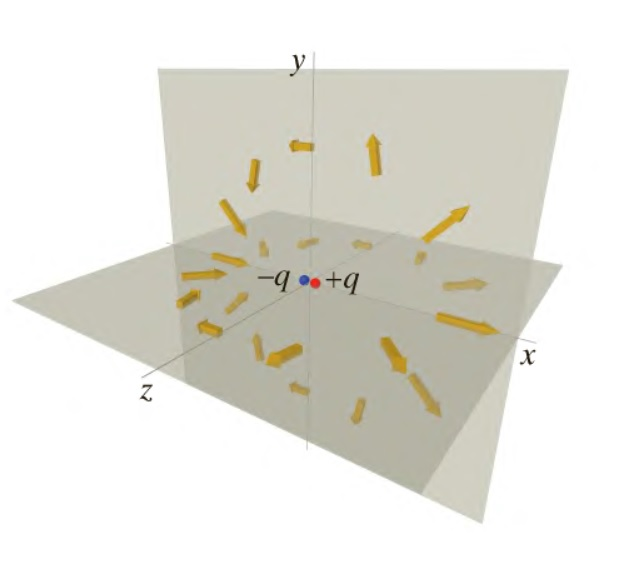
\includegraphics[width=0.5\linewidth]{images/dipole.jpg}
    \caption{دوقطبی الکتریکی}
    \label{fig:dynamicprogramming}
\end{figure}\\




